\subsection{Arbeitsaufteilung} \label{sec: einteilung}
\begin{tabular}{l | l | l | l}
\textbf{\nameSH} & \textbf{\nameJS} & \textbf{\nameCZ} &\textbf{\nameSB}\\
Projektleitung & Hardware & Hardware & Hardware\\
Hardware & Software & Software & Software\\
Software & & Steuerung & Testen \\
Steuerung & & Testen & \\
\end{tabular}
\vspace{3mm}
\subsection{Arbeitszeiten}
Die Arbeitszeiten wurden in Excel dokumentiert. Es wurde ein Kalender geführt, indem die Anzahl der Stunden und eine Beschreibung eingetragen wurden. In den unten abgebildeten Abbildungen werden die Arbeitsstunden aufgelistet. Es werden folgende Sachen mit den Abbildungen abgedeckt:
\begin{itemize}
    \item Arbeitsstunden pro Monat
    \item Gesamte Arbeitsstunden 
    \item Anzahl der Stunden Zuhause und in der Schule
\end{itemize}
\vspace{3mm}
\begin{table}[H]
    \centering
\begin{tabular}{ | l | c | c | c | c | c | c| c| } 
  \hline
  \textbf{ Name} & \textbf{September} & \textbf{Oktober} & \textbf{November} &\textbf{Dezember}&\textbf{Januar}&\textbf{Februar}&\textbf{März}\\
  \hline
    Sophia & 12 & 21 & 8 &20 & 28.5 &76.5&54\\ 
  \hline
    Julius & 16 & 40 & 24 &32 & 24 &23&31,5\\ 
  \hline
    Constantin & 12 & 15 & 15 &12 & 23 &24&64 \\  
  \hline
    Sebastian & 16 & 26 & 34 &25& 18 &31&11 \\ 
  \hline
\end{tabular}
    \caption{Stunden pro Monat}
\end{table}

\vspace{3mm}
\begin{table}[H]
    \centering
    \begin{tabular}{|c|c|c|}
    \hline
      \textbf{Name} & \textbf{Schule} & \textbf{Zuhause}\\
      \hline
       Sophia  & 80&140\\
       \hline
       Julius & 88& 102,5\\
       \hline
       Constantin &58&107\\
       \hline
       Sebastian&65&98\\
       \hline
    \end{tabular}
    \caption{Stunden Zuhaue und in der Schule}
    \label{tab:my_label}
\end{table}

\vspace{3mm}
\begin{table}[H]
	\centering
	\begin{tabular}{|c|c|c|}
		\hline
		\textbf{Name} & \textbf{Stunden}& \textbf{Prozentanteil}\\
		\hline
		Sophia  & 220& 30\%\\
		\hline
		Julius & 190,5&26\%\\
		\hline
		Constantin &165&22\%\\
		\hline
		Sebastian&163&22\%\\
		\hline
		Gesamt&738,5&100\%\\
		\hline
	\end{tabular}
	\caption{Gesamte Stunden}
	\label{tab:my_label}
\end{table}
\begin{figure}[H]
	\centering
	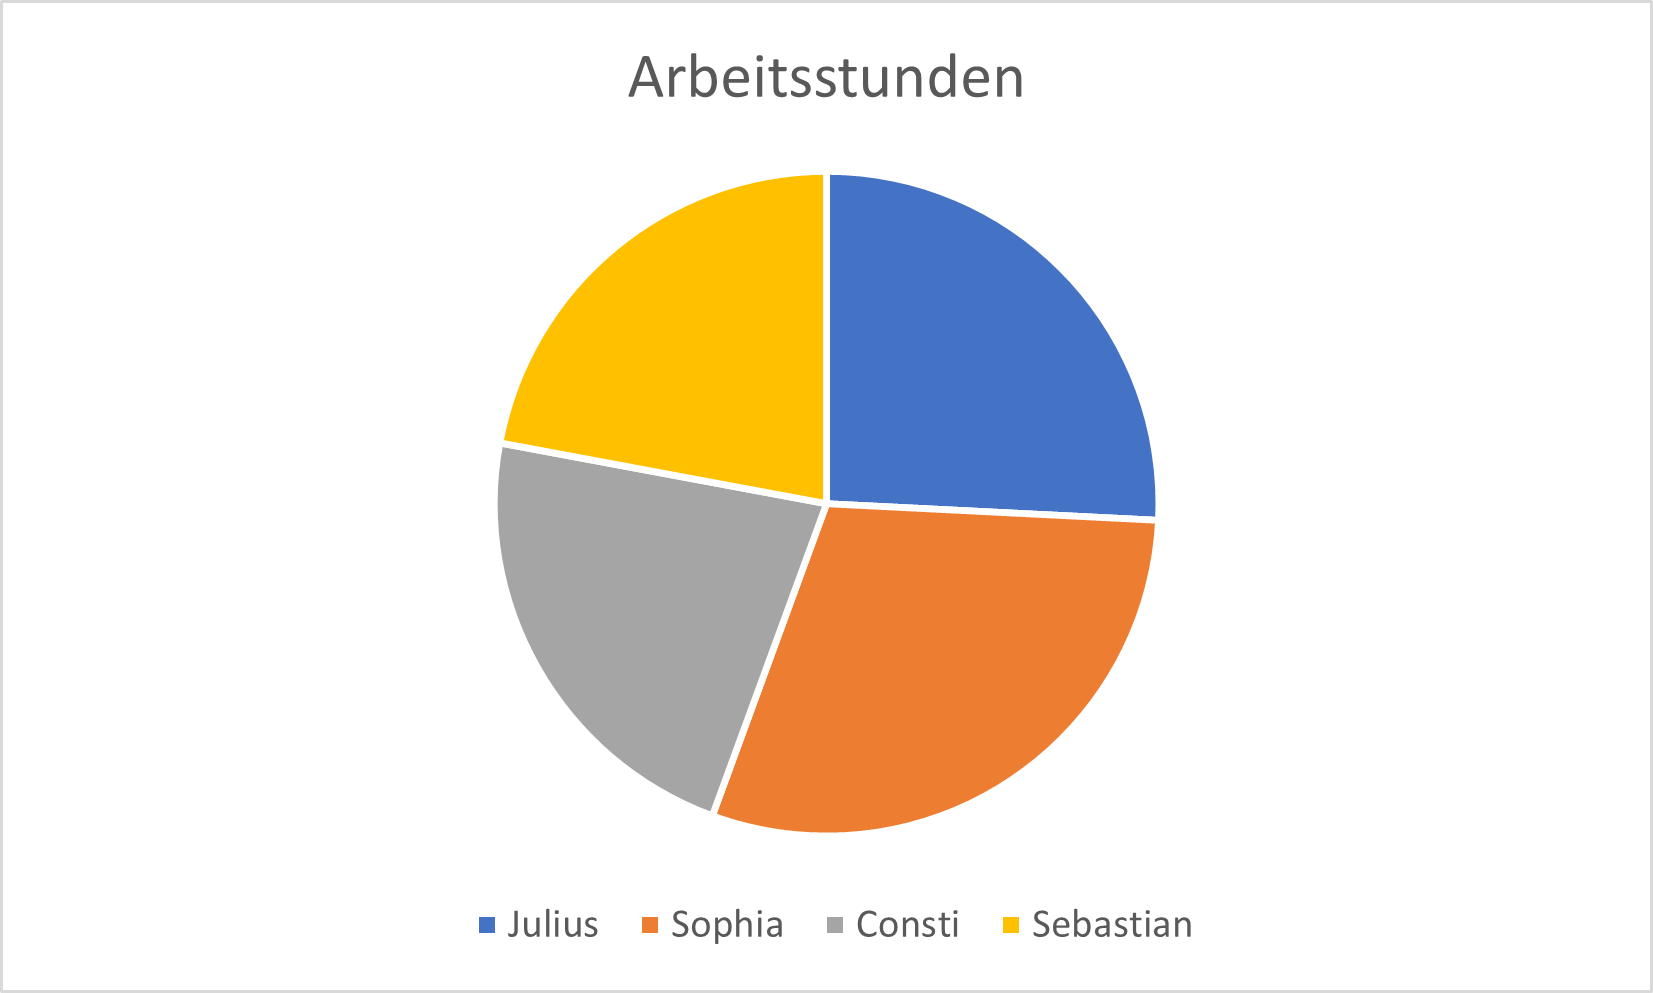
\includegraphics[scale=1.2]{image/graf.png}
	\caption{Aufteilung Arbeitsstunden}
	\label{fig:enter-label}
\end{figure}
